\documentclass[tcc]{ic}

\hypersetup{
    colorlinks = {true},
    linktocpage = {false},
    plainpages = {false},
    linkcolor = {Blue},
    citecolor = {Blue},
    urlcolor = {Red},
    unicode = {true},
    pdftitle = {Rapport d'activités en entreprise ADITU du 01-09-2023 au 13-09-2023}, 
    pdfauthor = {Alexis Déhu},
    pdfsubject = {Rapport de mes activités chez ADITU pour la période du 01-09-2023 au 13-09-2023},
    pdfkeywords = {activités, alternance, iut, but, rt, aditu, uppa, pau, bidart}
}

\usepackage{algorithm}
\usepackage{algpseudocode}

\makeatletter
\renewcommand{\ALG@name}{Algoritmo}
\renewcommand{\listalgorithmname}{List of \ALG@name s}
\makeatother

\newcolumntype{Y}{>{\centering\arraybackslash}X}

\begin{document}

    % Inclui o preâmbulo do documento (Informações da capa e contracapa)
    \titulo{Rapport d'apprentissage en entreprise}

\autor{Alexis Déhu}{a.dehu@aditu.fr}{}


\orientador{M. Éric Pierre-Sala}{}{}{}{}
%\orientador{Mr. Devesa Guillaume}{}{}{}{}
\examinador{M. Guillaume Devesa}{}{}{}{}

% \examinadorDois{Nome}{}{Instituto de Computação}{Universidade Federal de Alagoas}{Prof. Me.}

\dataMesAno{Septembre}{2023}{}

    \selectlanguage{english}
    
    % Capa, contracapa e avaliadores
    \capa

    % \aprovacao
    
    % Agradecimentos
    % \begin{agradecimentos}

Obrigado

\end{agradecimentos}
    
    % Resumo e Abstract
    \begin{resumo}
    Durant cette courte période de deux semaines, j'ai pris le temps d'apprendre un maximum sur le fonctionnement matériel et humain d'ADITU. Je pense désormais que cela a été essentiel pour l'obtention d'une bonne perspective de travail (ne pas avoir à revenir sur des notions que l'on m'aurait déjà expliquées, ou d'en avoir une vision erronée). Tout cela pour m'intégrer au mieux et commencer à travailler dans les meilleures conditions.
    \\ \\
    À l'issue de cette intégration, j'ai pu monter une infrastructure conteneurisée regroupant un ensemble d'outils destiné à accompagner l'équipe d'ADITU dans son travail. Cette initiation m'a permis une première prise en main de l'infrastructure informatique sans avoir à toucher à la criticité de la partie cliente. J'ai pu prendre en main les prémices de ce qui allait être mon travail quotidien.
    \\ \\
    Cette première période chez ADITU a été très enrichissante humainement - découverte des membres, des habitudes de travail - et techniquement - apprentissage des outils de l'entreprise, découverte des services, conceptualisation de solutions à la réponse de besoins -
    
    \palavrasChave{aimer découvrir; observation; écoute active; participation; communication; rédaction;}
\end{resumo}
    % \begin{abstract}
%     Lorem ipsum dolor sit amet, consectetur adipiscing elit. Duis elit tellus, vehicula in justo eget, fermentum aliquet nisi. In id quam mauris. Sed id vehicula libero. Quisque id tortor placerat, consequat ex sed, placerat ante. Ut dui nunc, placerat volutpat ipsum sit amet, dictum pellentesque lacus. Donec leo sem, dictum quis lacus at, ultricies sagittis elit. Mauris sit amet tortor efficitur, luctus justo sit amet, tincidunt tellus. Donec vulputate non risus at tincidunt. Sed accumsan at erat in aliquet. Sed consequat gravida bibendum. Sed fermentum metus sed ex lacinia mattis. Phasellus vel enim nisl. Proin tortor dui, luctus in erat a, dapibus convallis turpis. Maecenas vitae vulputate neque.

%     Etiam ac ante a lorem consectetur varius. Donec vitae dui porttitor, efficitur ante sed, aliquet lectus. Etiam aliquet mattis sagittis. Integer accumsan, est nec vehicula suscipit, nibh nisl varius ante, at convallis urna est dapibus massa. Orci varius natoque penatibus et magnis dis parturient montes, nascetur ridiculus mus. Praesent tempus dolor sit amet metus eleifend porta. Vestibulum eget viverra nulla. Mauris ac condimentum augue, quis molestie tortor. Duis ac condimentum tortor, sed ullamcorper nunc. Vivamus et suscipit arcu. Duis eget rutrum est, sed pellentesque leo. Nulla lorem lacus, faucibus vitae lectus eu, porttitor efficitur ante. Sed risus tortor, venenatis quis convallis non, blandit in orci. Morbi et neque hendrerit, consectetur magna vitae, consectetur dolor. Nam nec iaculis urna, vitae tincidunt eros. Ut pretium neque convallis turpis rutrum, nec dapibus est faucibus.
    
%     Quisque id laoreet ligula. In hac habitasse platea dictumst. Fusce scelerisque, nunc non lacinia maximus, lorem metus rutrum lacus, ac maximus dolor tellus at velit. Sed diam leo, interdum ut sapien at, finibus aliquam diam. Praesent vel erat id enim scelerisque fringilla. Aliquam cursus risus vulputate ex interdum, sit amet pretium augue semper. Curabitur eget risus eget nulla placerat ornare. Nam quis ornare ipsum. Duis id feugiat lectus. Phasellus vehicula leo id consequat porta. Aliquam ut massa malesuada, ultricies ipsum nec, euismod eros. In lacinia aliquet leo non mattis. Etiam semper neque risus, a condimentum diam euismod eget. Suspendisse vulputate viverra mauris, ac sollicitudin tellus placerat non. Nullam felis metus, congue sed neque ac, iaculis sollicitudin nisl.
    
%     \keywords{graphics processing; medical images; computer vision; deep learning; data augmentation;}
% \end{abstract}
    
    % Sumário
    \renewcommand*\contentsname{Table des matières}
    \tableofcontents
    \thispagestyle{empty}
    
    % Início dos capítulos
    \inicio
    
    \renewcommand{\figurename}{}
\mychapter{Premiers pas vers Aditu}{cap:premier_pas_vers_aditu} 
\lhead{Premiers pas vers Aditu}

Cette première partie aborde la présentation approfondie de l'entreprise ADITU, en y présentant son équipe, son secteur d'activité et les services en réponse; sa clientèle et enfin son périmètre d'attraction commerciale. Une deuxième sous-section est dédiée à mon intégration dans l'entreprise, traitant de mes conditions de travail et d'accueil, pour arriver sur la présentation d'une journée type de mes activités chez ADITU.

\section{Présentation d'Aditu}

ADITU est le nom de l'entreprise dans laquelle j'évolue dans mon alternance. Signifiant "écouter" ou "expert" en basque, elle se définit comme une société de prestation de services informatiques, ou ESN \textit{Entreprise de services du numérique}, à l'écoute de ses clients.
\\ \\
Elle fut fondée en 2004 en tant que première Délégation de Service Public en France dans le domaine des services aux entreprises. Sa création ayant été initiée par la Communauté d’Agglomération Côte Basque-Adour (Bayonne, Anglet, Biarritz, Boucau et Bidart). Son implémentation se fut à la Technopole Izarbel, à Bidart.
\\ \\
Toute son équipe, y compris son Dirigeant  Mr. Éric Pierre-Sala mon responsable, et son Directeur Technique Mr. Guillaume Devesa mon tuteur, m'ont accueilli dans leurs locaux.

\subsection{Secteur d'activité}

Le secteur d'activité d'ADITU se caractérise par sa réponse aux besoins d'aider les entreprises du secteur local à se développer plus rapidement et efficacement en les déchargeant de l'élaboration ou le maintient de leur infrastructure informatique. ADITU tend à être l'intermédiaire simple des professionnels locaux au monde du numérique.
\\ \\
ADITU participe au développement territorial en prenant en charge le déploiement et le maintient des infrastructures informatiques des acteurs locaux. Elle leur permet de pouvoir se concentrer sur leur activité en leur déchargeant de l'utilisation d'une infrastructure faillible ou incorrectement maintenue (complications au quotidien, perte de données, complexité d'utilisation, problème d'expansibilité multi-sites, failles de sécurités...).  
\\ \\
Le secteur d'activité est solide, assurant aux entreprises leur bon fonctionnement sans qu'elles aient besoin de former ou d'embaucher une personne technique à temps plein pour son infrastructure. L'équipe d'ADITU travail à la performance et à la refocalisation des entreprises sur leurs activités principales.

\subsection{Services proposés}

Pour répondre aux besoins du secteur d'activité, ADITU propose des services de conseils, d'installation et de maintient d'infrastructures informatiques à la demande pour ses clients. Chaque client peut choisir la souscription à un ou plusieurs services selon leurs besoins et le support souhaité.
\\ \\
Pour assurer la continuité des services proposés, ADITU possède deux datacenters \textit{centres d'hébergement et de gestion de données}, un premier à Bidart et un deuxième à Dax. Ces datacenters servent à \textbf{l'hébergement} de machines dédiées aux clients ou à l'hébergement de leurs services (sites WEB, service de messagerie, stockage et partage de fichiers, sauvegardes externalisées de postes ou de fichiers, applications en tout genre).
\\ \\
ADITU propose aussi la supervision du fonctionnement des services de ses clients, hébergés dans les datacenters ou sur leurs sites. Le service \textbf{d'infogérance} permet au client d'être informé en tant réel de la disponibilité de ses services pour ses collaborateurs, et d'être aussi rassuré de la remise en fonctionnement et du suivi de leurs services. L'infogérance englobe le support téléphonique et informatique, avec l'aide de résolution de problèmes au quotidien.
\\ \\
Pour répondre à la criticité des services de certains clients, l'infogérance peut être accompagnée d'une \textbf{astreinte} afin de garantir l'intervention sur incident dans les 45 minutes suivant la remonté de problème. Ce service est proposé avec un numéro d'appel, 365 jours par an, 24h sur 24, sans interruption. Ce service est d'une grande force pour les groupes voulant prouver leur professionalisme à leurs clients, par la haute disponibilité de leurs services et une réponse sur incident sûre.
\\ \\
Des journées en \textbf{régie} sont proposés, permettant l'envoi d'un technicien dédié au support et au contrôle du bon fonctionnement de l'infrastructure cliente sur l'ensemble d'une journée. Le technicien est alors solicité pour les problèmes mineurs, des formations sur équipements, de l'installation de nouveau matériel ou de la relation à client. Ce type de journées est intéressant pour de grands sites, permettant la vérification d'une utilisation propre de l'infrastructure installée, pour faciliter l'activité principale du client.

%Pour simplifier l'accessibilité mono-site ou multi-site

%pour répondre aux besoins du secteur d'activité... ; hébergement, infogérance, messagerie, sauvegarde externalisée, astreinte, régie

\subsection{Zone de chalandise}

ADITU a été fondé en soutient aux entreprises du Pays Basque, des Landes et du Béarn. Sa zone d'attraction s'étend dans ces régions. Cette zone de chalandise reste locale mais très éclatée sur la côte Basque. Le Directeur d'ADITU, Mr. Pierre-Sala Éric, désir que l'entreprise garde cette zone de chalandise pour conserver la proximité avec ses clients et ses acteurs, afin de conserver une relation humaine avec eux.
\\ \\
ADITU n'est pas la seule entreprise dans son secteur d'activité à s'intéresser à cette zone de chalandise. Celle-ci possède de nombreux concurrents, de même ou plus grande envergure. La zone de chalandise se retrouve ainsi divisée entre les imposants groupes proposant des services de plus grande échelle, et les groupes de taille humaine comme ADITU ayant de la proximité avec ses clients et étant appréciés pour leur localité.

% Clients locaux (pays basques, landes); 

\subsection{Clientèle ciblée}

La clientèle ciblée par la zone de chalandise est variée, regroupant entreprises et organisations ayant besoin d'externaliser la gestion de leur infrastructure numérique. La plupart des clients d'ADITU sont des clients "historiques" avec plus de dix années d'ancienneté.
\\ \\
Les clients d'ADITU sont des clients souhaitant de la proximité et de l'humain pour leur informatique, pouvant parler avec une personne. Ces personnes veulent de la proximité, étant généralement attachés à leur région - de par leur activité ou leur clientèle, et sont demandeurs d'acteurs locaux.
\\ \\
La différence de taille parmis les groupes des clients reste considérable : pouvant aller d'un grand groupe souhaitant s'installer dans le pays basque à une TPE \textit{Très Petite Entreprise} dans le besoin de quelques services.

% clients "historiques"; ceux qui ne veulent pas payer une fortune dans office365; ceux qui veulent avoir de la proximité; les gens attachés à leur secteur et demandeurs d'acteurs locaux

\section{Encadrement dans l'entreprise}

Cette deuxième sous-section est consacrée à mon encadrement dans l'entreprise. Celle-ci y aborde mes conditions générales de travail chez ADITU (temps de travail, organisation, relation à clients et collègues, encadrement pour l'alternance...) ainsi que mon environnement quotidien de travail (type de bureau, matériel, déplacement...). Je finis par présenter une visualisation d'une journée type de travail. 

\subsection{Conditions de travail}

Spécifié dans mon contrat d'alternance, mon lieu de travail se situe dans les bureaux d'ADITU à Bidart, Pavillon Izarbel. J'y travaulle du lundi au vendredi de 9h à 12h, puis de 14h 18h. J'y retrouve mon responsable Éric, mon tuteur Guillaume ainsi que mes collègues ces mêmes jours.
\\ \\
L'organisation de la semaine prend place le lundi matin aux environs de 9h30, par une réunion technique et une autre d'exploitation. Ces réunions ont pour objectifs respectifs de définir l'état d'avancement des projets de chacun et la planification de leurs tâches pour la semaine. Les alternants participent à ces réunions au même titre que les autres membres de l'équipe.
\\ \\
J'ai souvent eu l'occasion de discuter avec mon tuteur Guillaume ou mon responsable Éric, en essayant le plus possible de ne pas empiéter sur leurs temps de travail respectifs. Je suis convié une fois par période d'entreprise à faire un point avec eux sur ma situation personnelle, professionnelle et scolaire. Nous parlons fréquemment entre collègues du même service. Je n'ai eu que rarement l'occasion de converger avec des clients (voir Première activités).
\\ \\
J'ai effectué une visite médicale du travail la première période en entreprise le 12 septembre 2023 à 11:30.

\subsection{Environnement de travail}

L'environnement de travail est propre et sécuritaire. Mon activité principale respose sur l'utilisation d'un poste de travail fixe, faisant partie du NOC \textit{Network Operations Center} d'ADITU. L'agencement du NOC forme un open space collaboratif. Certaines tâches m'ont demandé d'aller dans le datacenter d'ADITU pour des manipulations, sous surveillance et explications les premières fois.
\\ \\
Je n'ai pas besoin de me déplacer dans mon travail, je ne fais pas de clientèle commerciale ou technique, ni de manipulations sur le datacenter de Dax. J'ai l'occasion de questionner les membres de l'équipe sur des spécificités, de l'aide ou des conseils (toujours en essayant de leur emprunter la période de temps la plus courte pour ce qui est demandé).

\subsection{Journée type}

Avec la réunion technique et celle d'exploitation le lundi, mes journées se déroulent dans les bureaux d'ADITU, sur mon poste ou dans son datacenter. J'y effectue mes tâches mises au point la veille, entouré des autres personnes de l'équipe.
\\ \\
Le travail qui m'est demandé est souvent encadré par un cahier des charges à mon retour de période scolaire. J'y découvre mes activités pour la période d'entreprise, faisant des mises aux points régulières les lundi matin.
    \mychapter{Premières activités}{cap:premieres-activites}
\lhead{Premières activités}

Cette deuxième section est dédiée au compte rendu de mes activités et de mon apprentissage faits pendant cette première période dans l'entreprise. Celle-ci intègre ma prise de connaissance du fonctionnement global de la structure, avec l'exposition dans l'état des premiers projets qui m'ont été confiés.  

\section{Prise de marques}

Une grande partie de mon apprentissage pendant ces deux premières semaines s'est dévouée à la considération et à l'intégration du fonctionnement informatique et humain de la structure. Connaître l'environnement logique et opérationnel de son infrastructure est fondamental pour initier une perspective de travail. À contrario de travailler seul, sur son propre équipement, pour son intérêt personnel.

%Avant de pouvoir travailler dans une infrastructure, il est fondamental de connaître son fonctionnement logistique \& opérationnel avant d'initier une procédure de mise en oeuvre.

\subsection{Découverte du fonctionnement de l'infrastructure}

Le service technique comporte les techniciens informatique, les administrateurs systèmes et réseaux \& son directeur technique. Les techniciens informatique sont davantage sollicités pour la manipulation ou l'installation d'appareils chez les clients ou dans les datacenters, ainsi que pour le support et la réparation de matériel.
\\ \\
Les administrateurs élaborent le déploiement de ces équipements, planifient leur maintenance et les administrent depuis le NOC. Le directeur technique orchestrant l'ensemble de ces activités, en plus de travailler comme administrateur systèmes \& réseaux de longue date. Les alternants se formant à prochainement devenir des administrateurs systèmes et réseaux.
\\ \\
Les tâches de chacun vis-à-vis des clients sont définies et expliquées dans des \textbf{bons de travaux}, avec des \textbf{bons de livraison} lorsqu'une installation d'équipement doit être faite. Les devis, facturations, gestion des clients et des prospects sont fait par Mr. Pierre-Sala Éric.
\\ \\
À notre arrivée, des \textbf{fiches de postes} ainsi que des cahiers des charges nous ont été confiés pour nous encadrer dans les projets attendus et notre alternance. Ces fiches sont aussi présentes chez les autres corps de métiers pour encadrer leurs activités.

% dire que ces deux premières semaines on a beaucoup questionné sur les hyperviseurs, le réseau...

%réu exploit + technique; comment l'organisation se fait (prestations, bons de travaux, bons de livraisons, devis, fiches de postes); nos accès; noc; hyperviseurs esxi; réseau d'un "datacenter"; prise de connaissance des bonnes pratiques

\subsection{Accoutumance aux bonnes pratiques}

Chaque entreprise a ses habitudes dans son fonctionnement, via leurs applicatifs ou leur méthodologie (gestion des documentations, de l'archivage, des applicatifs, des sauvegardes)... Cela peut aussi s'appliquer à la nomenclature des systèmes, l'arborescence des fichiers... Il m'a paru essentiel d'assimiler les bonnes pratiques de l'entreprise pour m'y intégrer au mieux : le travail y sera plus agréable pour moi et pour les autres.
\\ \\
Ainsi, à mon arrivée, une fiche d'intégration m'a été distribuée avec mes premiers identifiants de connexion pour les applicatifs communs. J'ai ainsi compris par déduction que le nom des sauvegardes, la rédaction des procédures ou la nomenclature des hôtes étaient réglementées et normalisées : je m'y suis tout de suite adapté.
\\ \\
D'autres domaines comme des astuces ou des coups de pouces n'étaient pas explicités. Je les ai découvert notamment lors d'explications de mon travail aux autres personnes de l'équipe, lorsque celles-ci m'expliquaient comment j'aurais pu simplifier mon travail en effectuant des actions différemment avec certains outils. L'accoutumance à une entreprise passe aussi par une bonne prise en main de ses outils.
\\ \\
Cette accoutumance aux applicatifs, aux astuces de certains logiciels ou autres manières de réfléchir à son travail m'ont beaucoup aidés à prendre mes marques les premières semaines.

\section{Mise en place de services internes}

Pour la première prise en main de l'infrastructure, le cahier des charges demandait l'installation de solutions pour l'amélioration, la simplification ou l'ajout de fonctionnalités au travail général de l'équipe d'ADITU. Ainsi, sans avoir à toucher à la criticité de l'infrastructure des clients, j'ai mis en place plusieurs services internes à ADITU.

\subsection{Aménagement d'un environnement conteneurisé}

Les services reposent sur un environnement conteneurisé Docker. Cela minimise les ressources nécessaire par service, augmente la reproductibilité et l'ensemble des solutions devient plus flexible. Pour simplifier la manipulation des ressources Docker (conteneurs, images, volumes, réseaux), une interface graphique intuitive a été montée, permettant le dépannage rapide des solutions - redémarrage en un clique, diagnostique rapide par indicateurs lumineux...
\\ \\
L'ensemble de cette solution repose sur une machine virtuelle \textit{VM}, hébergée sur un hyperviseur.

\subsection{Installation d'un proxy inverse}

L'ensemble des services ont été montés derrière un proxy inverse \textit{reverse proxy}. Un proxy normal permet la centralisation des points de sortie web pour Internet, pour les faire passer par un uniquement équipement. Utile pour restreindre l'accès à certains site, permettre la mise en tampon de pages web entre utilisateurs, ou pour la rétention d'activités globales sur le web.
\\ \\
Le proxy inverse permet la centralisation des accès et le déploiement de plusieurs services derrière une machine avec la même adresse IP. Le principe est identique au proxy simple, mais dans l'autre sens : au lieu de centraliser les points pour sortir vers Internet, il démultiplexe l'arrivée pour les services voulus. Selon le lien \textit{URL} contacté, le proxy inverse redirige l'activité pour le service voulu, en ayant toutes les URL dirigeant vers la même adresse IP.

\begin{figure}[H]
    \centering
    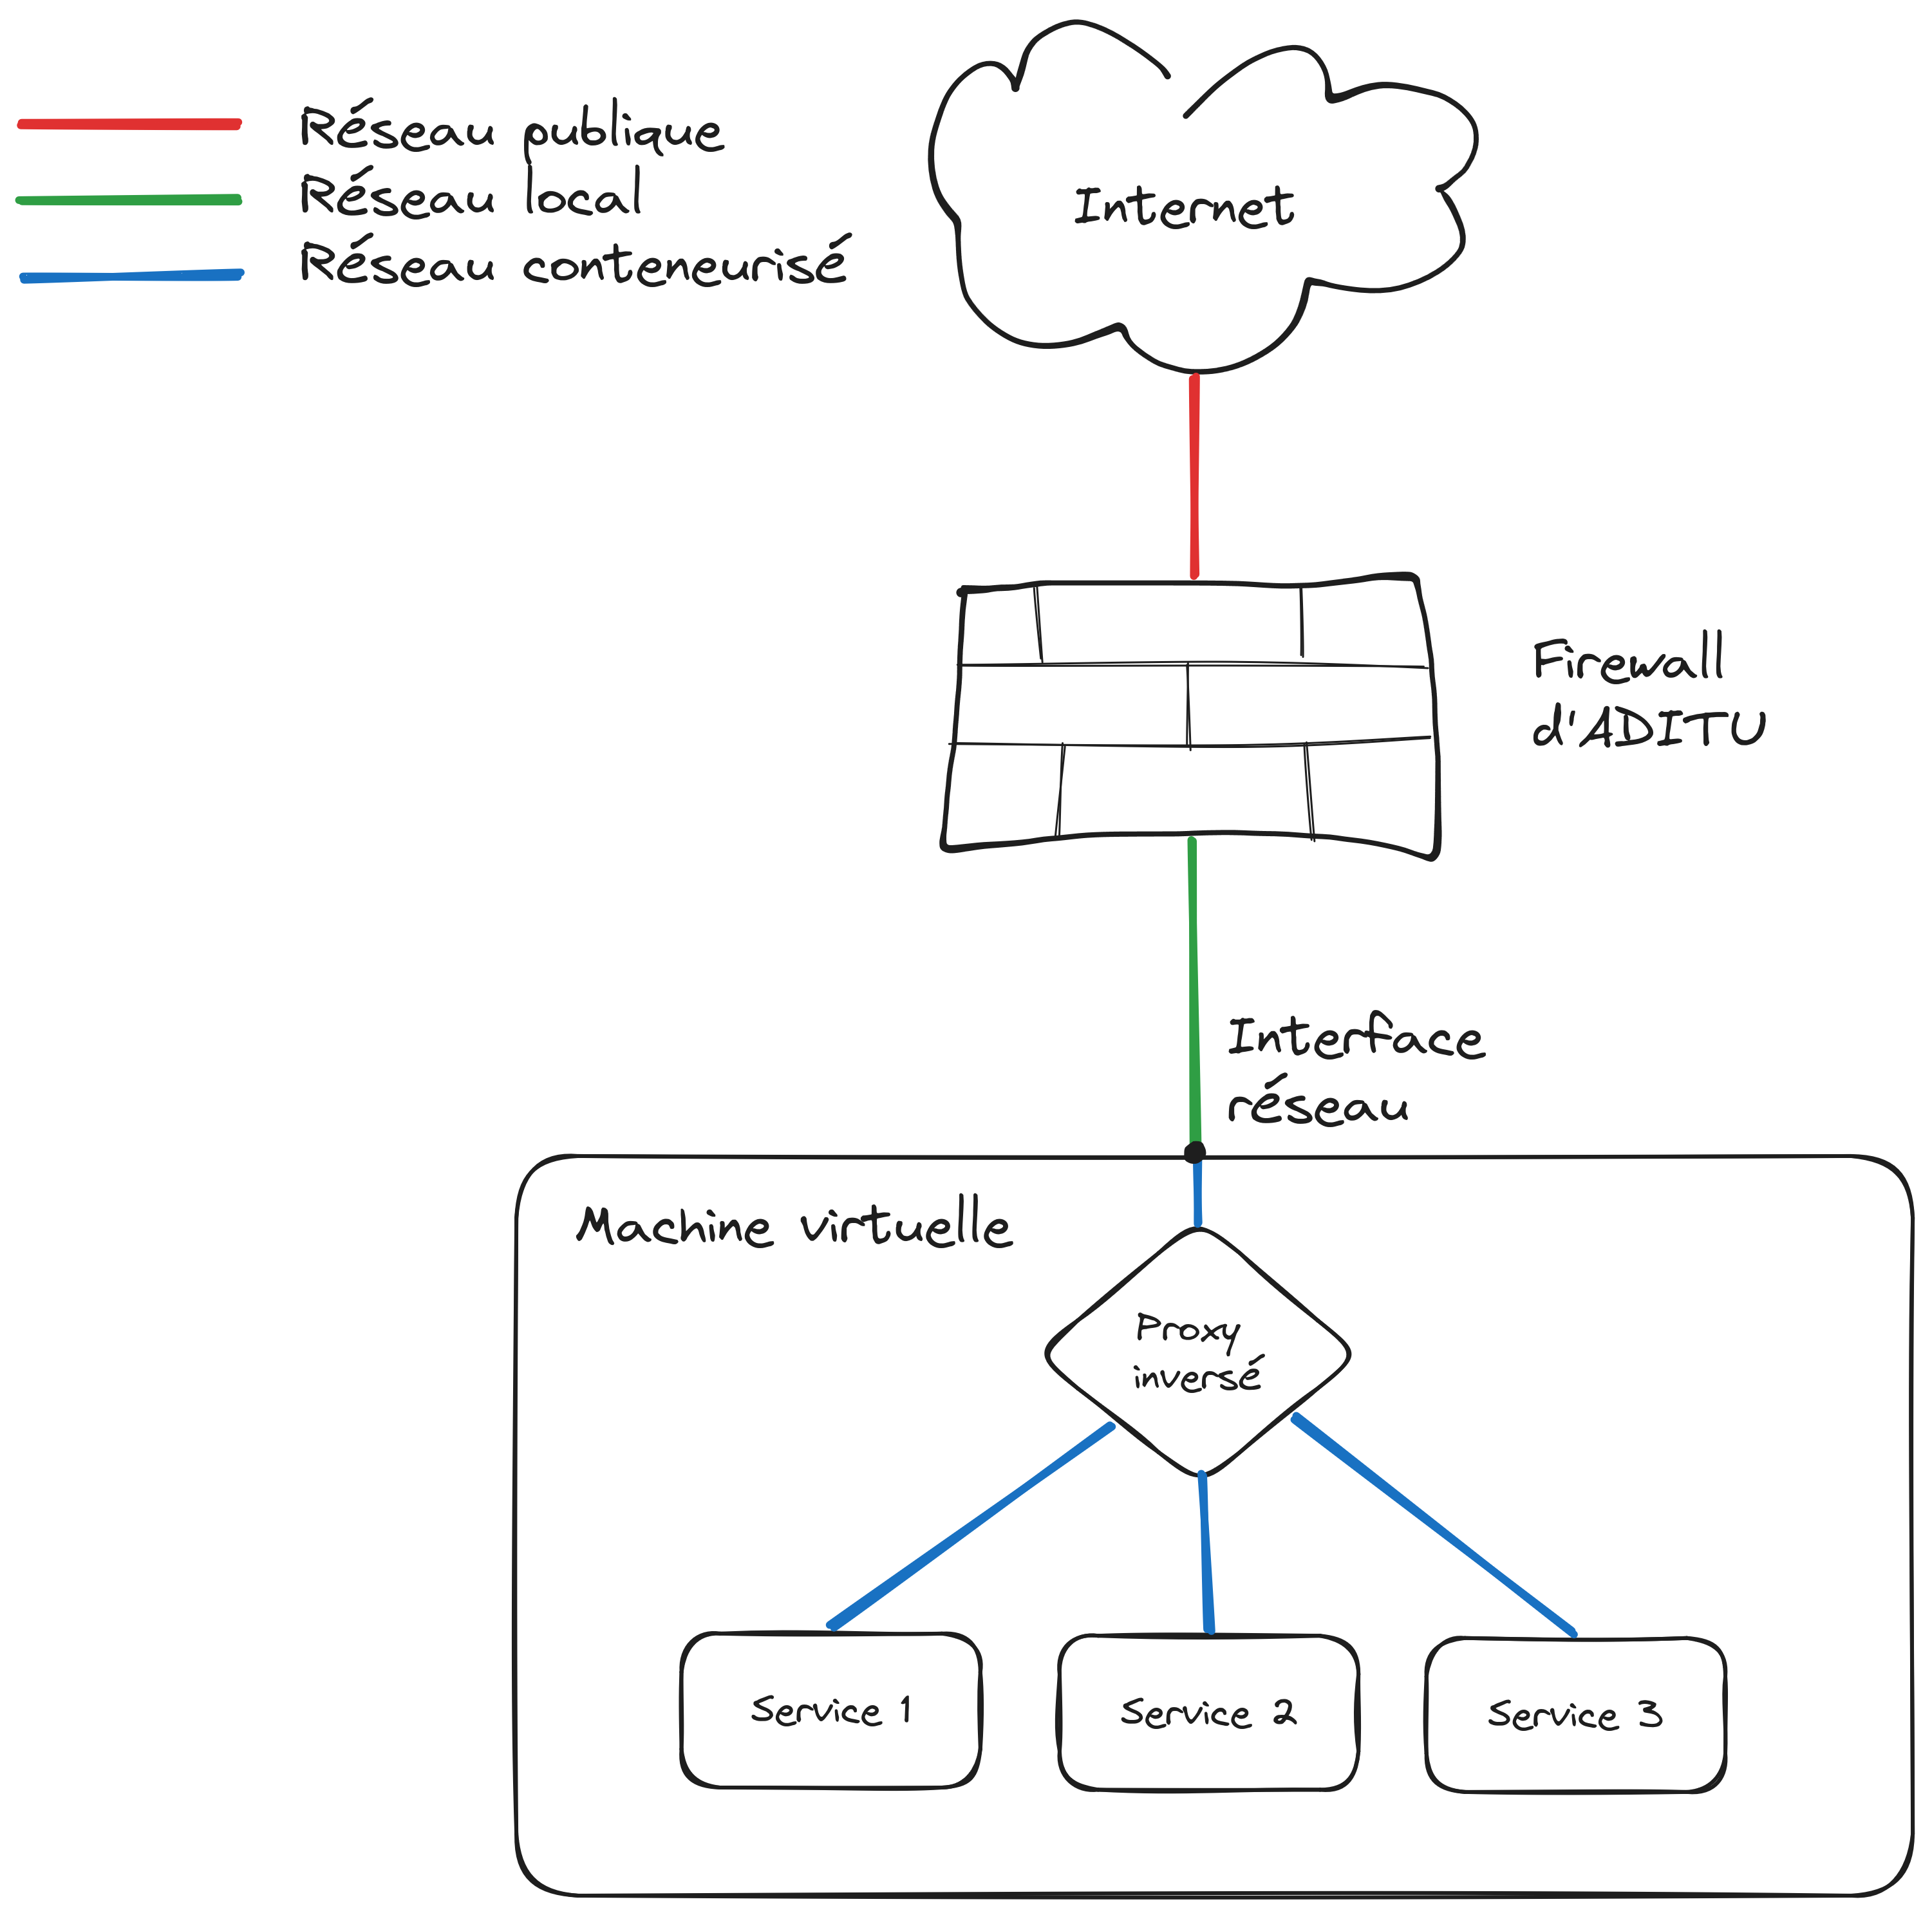
\includegraphics[width=\textwidth - \textwidth / 6]{Untitled-2024-01-21-1259.png}
    \figurename
    \caption{Vision d'esprit simplifiée du proxy inverse}
    \label{fig:rvproxy}
\end{figure}

\noindent Cette manipulation permet l'hébergement de plusieurs services, par communication sur le même port, en n'utilisant qu'une seule adresse IP publique - précieuse car chères à l'achat. La différenciation du service voulu s'effectuant par l'identification de l'URL renseigné.
\\ \\
Le proxy inverse gère les certificat SSL/TLS pour les services qu'il redirige (la sécurisation du traffic), ainsi que le contact des ports. Les services peuvent être hébergés sur une autre machine, à condition que le proxy inverse puisse la contacter sur le port pour communiquer avec le service hébergé.

% explication utilité reverse proxy pour ce qui va arriver après (une ip publique); schéma; donner le nom de la solution

\subsection{Montage d'un service de partage d'informations sécurisé}

Le premier service monté derrière le proxy inverse fut un service de partage d'informations sécurisé. Celui-ci prend place lors d'échange de mots de passe ou de lignes de configuration avec des clients. ADITU peut en envoyer aux clients comme l'inverse.
\\ \\
Au lieu d'envoyer des mots de passe ou des fichiers de configuration par mails, ceux-ci sont regroupés sur une plateforme accessible par l'attendu uniquement (authentification + autorisation). Cette plateforme permet la non divulgation d'informations sensibles par mail (mots de passe, informations sensibles...), leur chiffrement et un accès sécurisé.
\\ \\
Des mesures de sûreté sont mises en place : possibilité de suppression de l'information après première lecture, confirmation de la lecture, temps limite d'accessibilité à la ressource (utile pour les mots de passe qui "ne doivent pas trainer").
\\ \\
Une solution similaire de secours est aussi mise en place. La première étant traduite en français pour un usage primaire et globale.

%mots de passe et fichier de conf

%expliquer pourquoi besoin de ne pas donner mot de passe en clair dans message (un mec vient, récupère; si self-host, un mec vient, galère et par chance abandonne); envoi de fichiers de configuration par yopass; partage avancés de mots de passe pwdpush (voir si personne à vu et quand, temps maximal, accès une fois)

\subsection{Implémentation d'une solution de partage de fichiers volumineux}

Aucune solution de partage de fichiers volumineux n'était présente chez ADITU. Ainsi, le transport manuel ou par hébergeurs tiers étaient nécessaire pour le transfert de fichiers lourds (fichiers compressés, export de boites mail, enregistrement de caméras...).
\\ \\
Une solution de partage de fichiers volumineux a été monté derrière le proxy inverse pour permettre à ADITU et à ses clients de pouvoir y déposer des fichiers \& de pouvoir les partager. Cette solution est davantage professionnel, plutôt que de passer par des services tiers (Google Drive, Microsoft OneDrive...). De plus, celle-ci est hébergée chez ADITU et bénéficie de la sécurité \& la gestion de son réseau.

\subsection{Déploiement d'une console de vérification de disponibilité}

Le centre de donnée de Dax est certifié ISO 27001 HDS pour l'hébergement de données de santée (pour les hôpitaux...). Cette certification demande des tests périodiques de bascule de réseaux d'opérateurs (accès à Internet) et de restauration de sauvegarde.
\\ \\
Le test de bascule d'opérateur revient à simuler la coupure d'un lien vers Internet pour s'assurer que le datacenter soit toujours accessible depuis l'extérieur en basculant sur un lien de secours - haute disponibilité. Pour s'assurer du bon fonctionnement du test de bascule d'opérateur, une console de vérification de l'état des services a été montée, toujours derrière le proxy inverse.
\\ \\
Cette console vérifie en temps réel la disponibilité des services hébergés dans le datacenter de Dax depuis celui de Bidart. Ainsi, lors de la bascule d'opérateur à Dax, les services sont indisponibles pendant un très court instant pendant que les équipements du datacenter adapte leur configuration pour la nouvelle route - selon l'activité, indistinguable par l'utilisateur.
\\ \\
Le rôle de cette console est de superviser la disponibilité des service hérbergés à Dax, utile lors du test de bascule pour vérifier l'accessibilité des services depuis l'extérieur.

% expliquer pourquoi besoin de se simplifier et pas à avoir à génerer des accès à chaque fois; fichier de conf importants parfois mots de passes dedans ou informations sensibles
    \mychapter{Annexes}{cap:annexes}
\lhead{Annexes}

Regroupement des documents servant à l'appui des éléments cités précédemment. Pouvant être de toutes formes (images, blocs de texte, photos...).

\section{Cahier des charges supervision}

Cahier de charges supervision

La recherche de solution applicative de supervision devra se base au
minimum sur deux applications pour avoir une comparaison objective.

Voici les fonctionnalités souhaitées~:

\ul{Serveurs Proxy}

L'utilisation de \textbf{SERVEUR PROXY} pour ne pas avoir un seul
serveur qui se charge de l'ensemble de vérifications de sonde.

\ul{DASHBOARD}

Un \textbf{DASHBOARD UNIQUE} qui inclut l'ensemble des serveurs de
supervision.

\ul{DASHBOARD TV}

Un \textbf{DASHBOARD} pour la télé qui liste les notifications de la
plus récente a la plus ancienne. (Comme celle que l'on a actuellement.)

\ul{Type de contrôles}

L'application devra gérer les contrôles \textbf{PASSIF} et
\textbf{ACTIF} et la prise en charge des contrôles via \textbf{SNMP}.

\ul{Type de paramétrages}

La possibilité de configurer les hosts via l'interface graphique et via
les fichiers de configuration.

Exemple~: sur l'ancienne supervision on créer un fichier de conf par
client.

\ul{Notifications}

Les notifications devront être effectuées par mail et par SMS tout en
ayant une gestion des utilisateurs et des groupes (possibilité
d'intégrer la solution à notre serveur d'SMS)

Déplacer le GSM dans le bureau ADITU de Pulseo pour une meilleur
couverture réseau (prévoir onduleur + switch mangeable)

\ul{Accès restreint client}

Donner la possibilité à certains clients de visionner leur supervision
en lecture et d'être alerté par mail.

\ul{Graphique}

Côté graphique, il serait bien que la solution puisse avoir la
possibilité d'inclure les graphiques comme fait Cacti pour éviter
d'avoir 2 solutions.

\begin{itemize}
\item
  Graphique réseau
\item
  Graphique volumétrie disque pour voir l'évolution du stockage
\item
  Graphique mémoire ou CPU
\end{itemize}

\ul{Tarif}

Open source gratuit

% \begin{figure}[H]
%     \centering
%     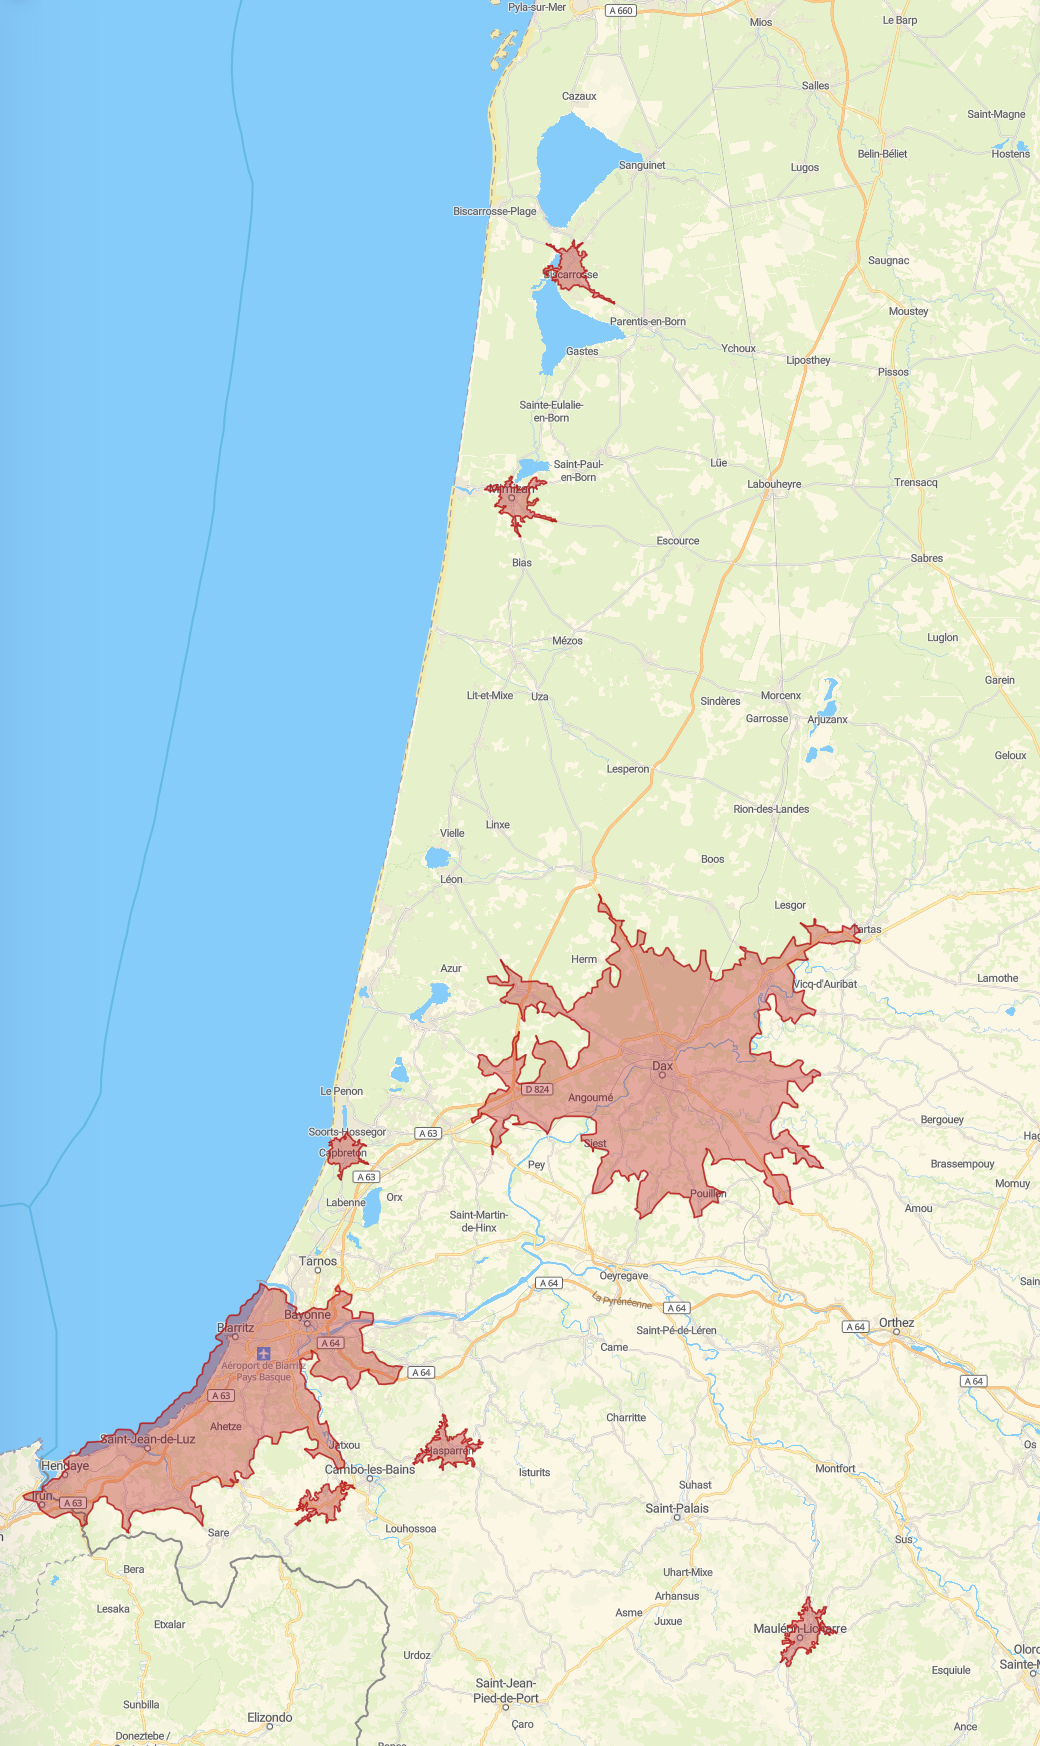
\includegraphics[width=\textwidth - \textwidth / 5]{zone_chalandise_aditu.png}
%     %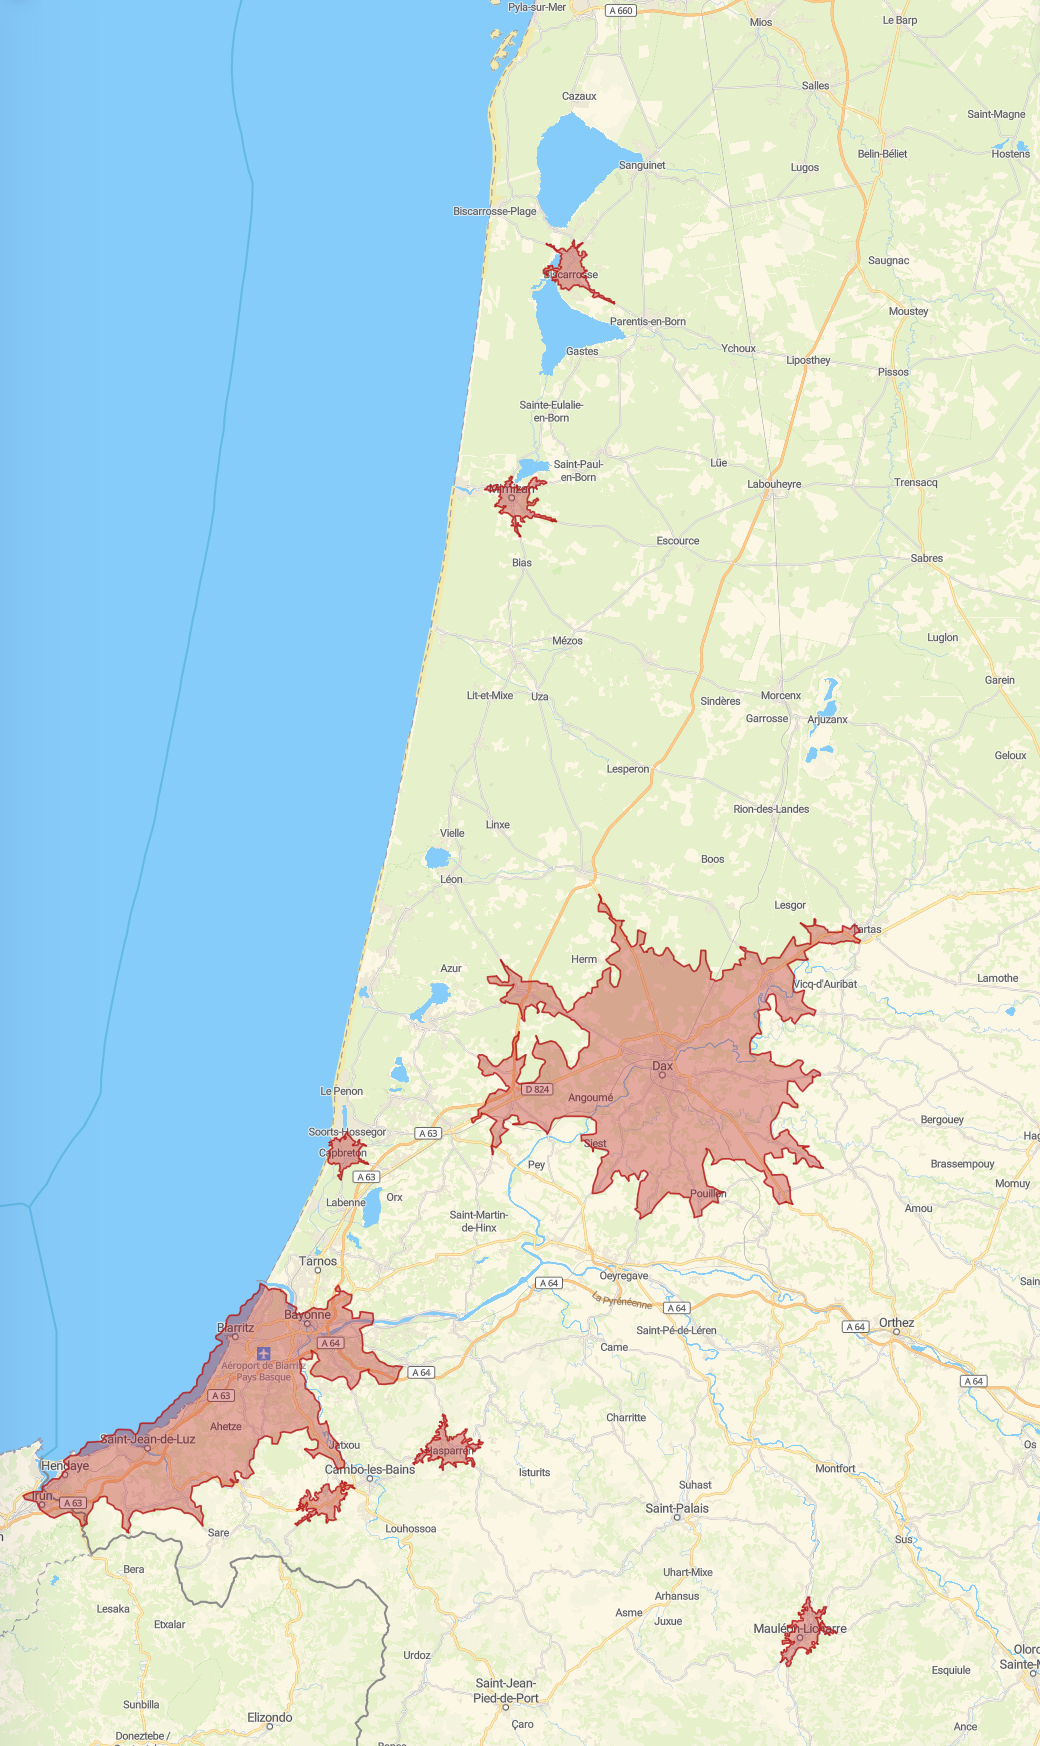
\includegraphics[scale=0.2]{zone_chalandise_aditu.png}
%     \figurename
%     \caption{Visualisation de la zone de chalandise d'ADITU, regroupée autour de ses datacenters à Bidart et à Dax}
%     \label{fig:zone_chalandise}
% \end{figure}

% \section{Cahier des charge Ticketing}

% % \begin{figure}[H]
% %     \centering
% %     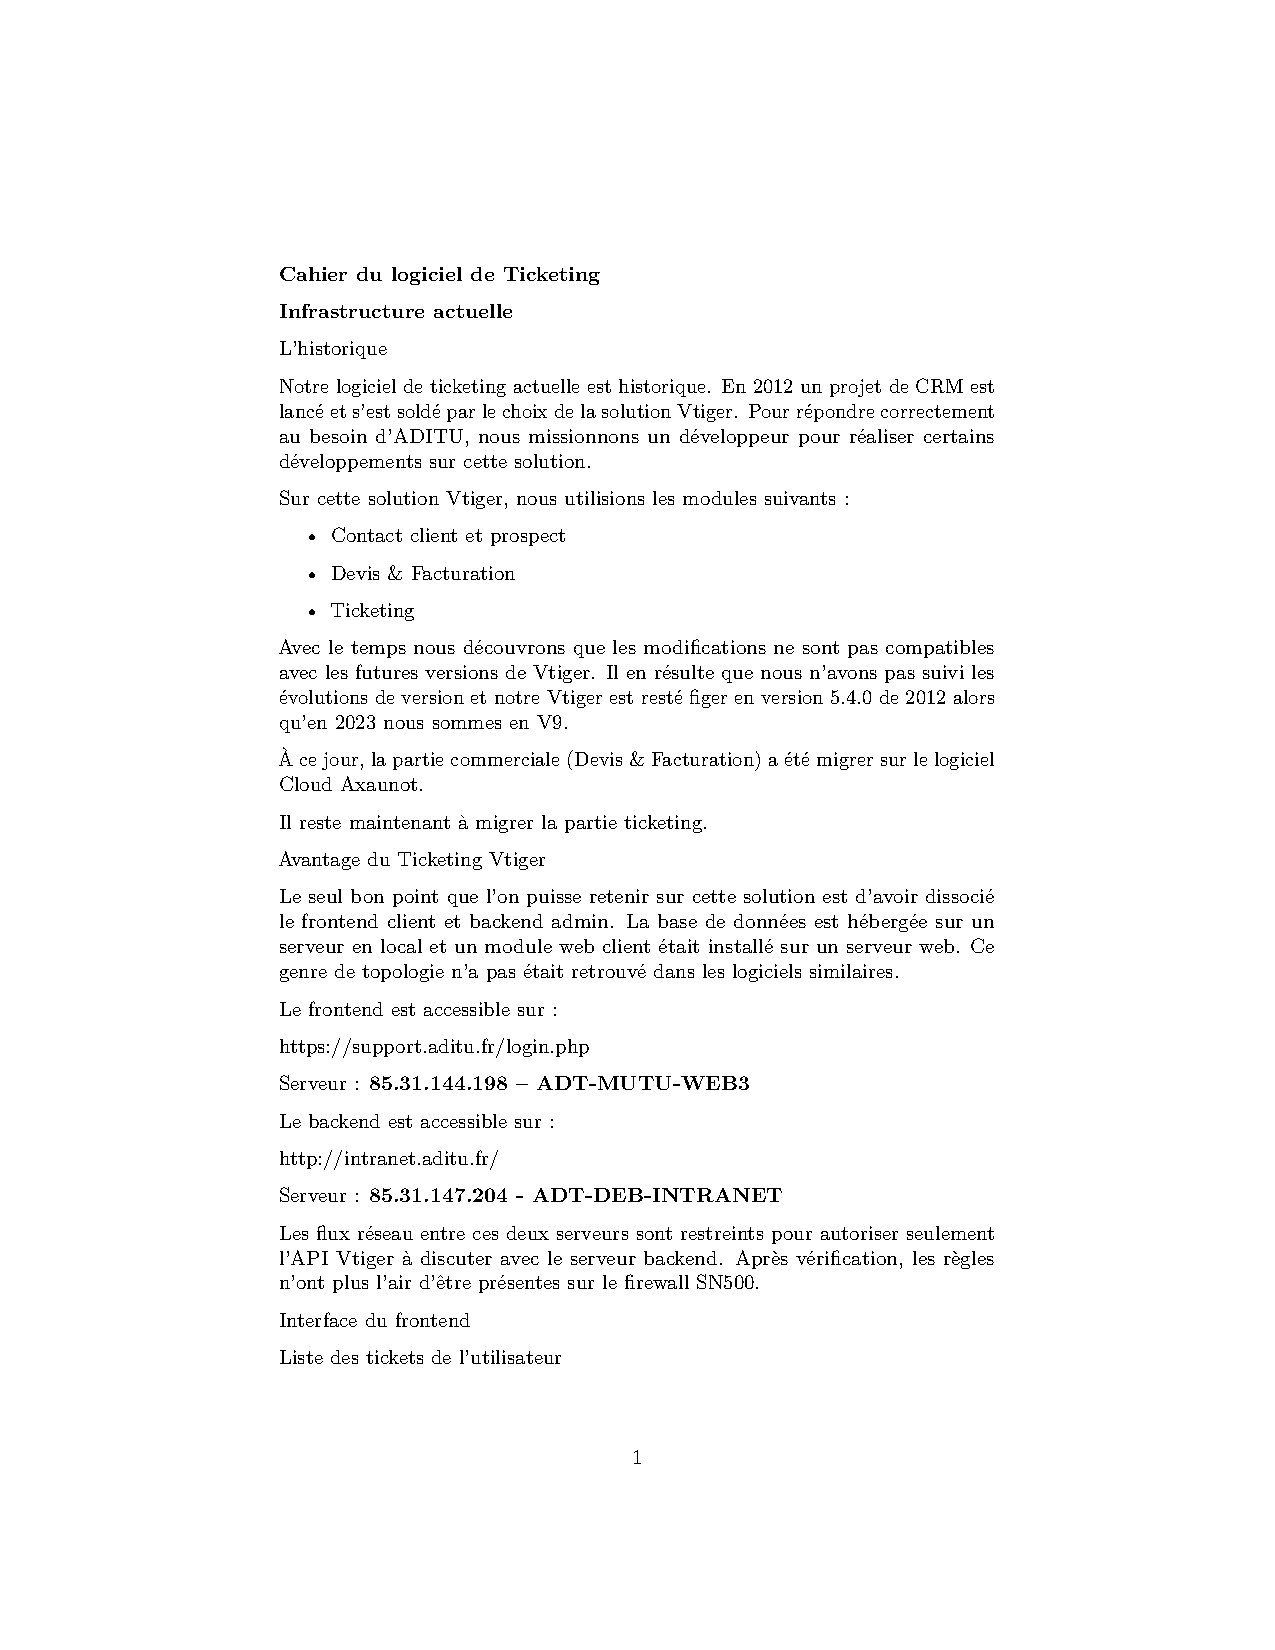
\includegraphics[width=\textwidth - \textwidth / 20]{CDC-Ticketing.pdf}
% %     \figurename
% %     \caption{Fiche de poste de notre alternance}
% %     \label{fig:poste}
% % \end{figure}

% \textbf{Cahier du logiciel de Ticketing}

% \textbf{Infrastructure actuelle}

% L'historique

% Notre logiciel de ticketing actuelle est historique. En 2012 un projet
% de CRM est lancé et s'est soldé par le choix de la solution Vtiger. Pour
% répondre correctement au besoin d'ADITU, nous missionnons un développeur
% pour réaliser certains développements sur cette solution.

% Sur cette solution Vtiger, nous utilisions les modules suivants~:

% \begin{itemize}
% \item
%   Contact client et prospect
% \item
%   Devis \& Facturation
% \item
%   Ticketing
% \end{itemize}

% Avec le temps nous découvrons que les modifications ne sont pas
% compatibles avec les futures versions de Vtiger. Il en résulte que nous
% n'avons pas suivi les évolutions de version et notre Vtiger est resté
% figer en version 5.4.0 de 2012 alors qu'en 2023 nous sommes en V9.

% À ce jour, la partie commerciale (Devis \& Facturation) a été migrer sur
% le logiciel Cloud Axaunot.

% Il reste maintenant à migrer la partie ticketing.

% Avantage du Ticketing Vtiger

% Le seul bon point que l'on puisse retenir sur cette solution est d'avoir
% dissocié le frontend client et backend admin. La base de données est
% hébergée sur un serveur en local et un module web client était installé
% sur un serveur web. Ce genre de topologie n'a pas était retrouvé dans
% les logiciels similaires.

% Le frontend est accessible sur~:

% \url{https://support.aditu.fr/login.php}

% Serveur~: \textbf{85.31.144.198 -- ADT-MUTU-WEB3}

% Le backend est accessible sur~:

% \url{http://intranet.aditu.fr/}

% Serveur~: \textbf{85.31.147.204 - ADT-DEB-INTRANET}

% Les flux réseau entre ces deux serveurs sont restreints pour autoriser
% seulement l'API Vtiger à discuter avec le serveur backend. Après
% vérification, les règles n'ont plus l'air d'être présentes sur le
% firewall SN500.

% Interface du frontend

% Liste des tickets de l'utilisateur

% 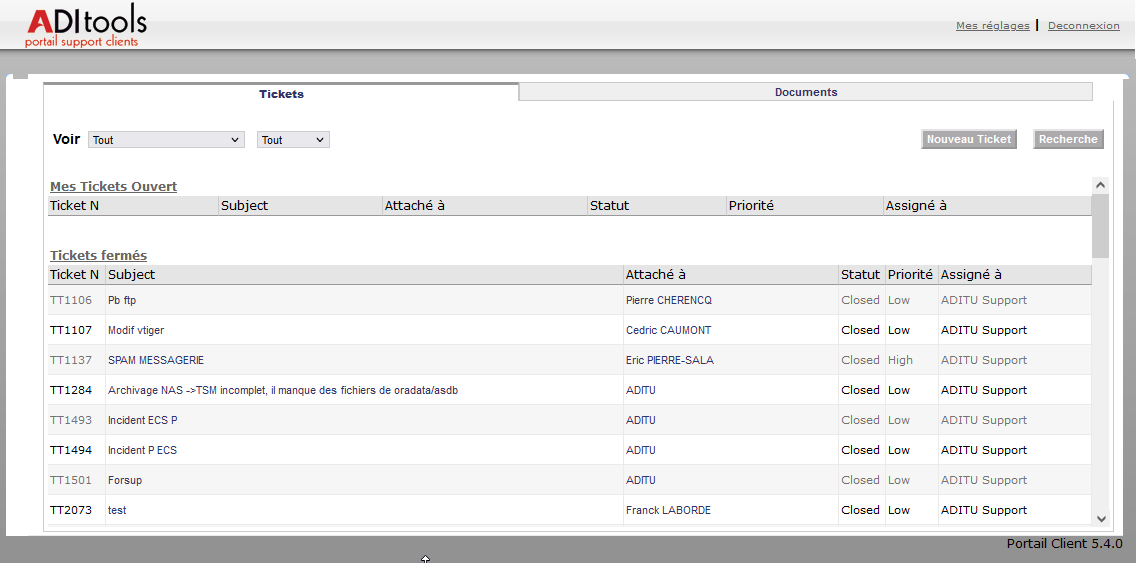
\includegraphics[width=6.3in,height=3.12222in]{image1.png}

% Création de tickets

% 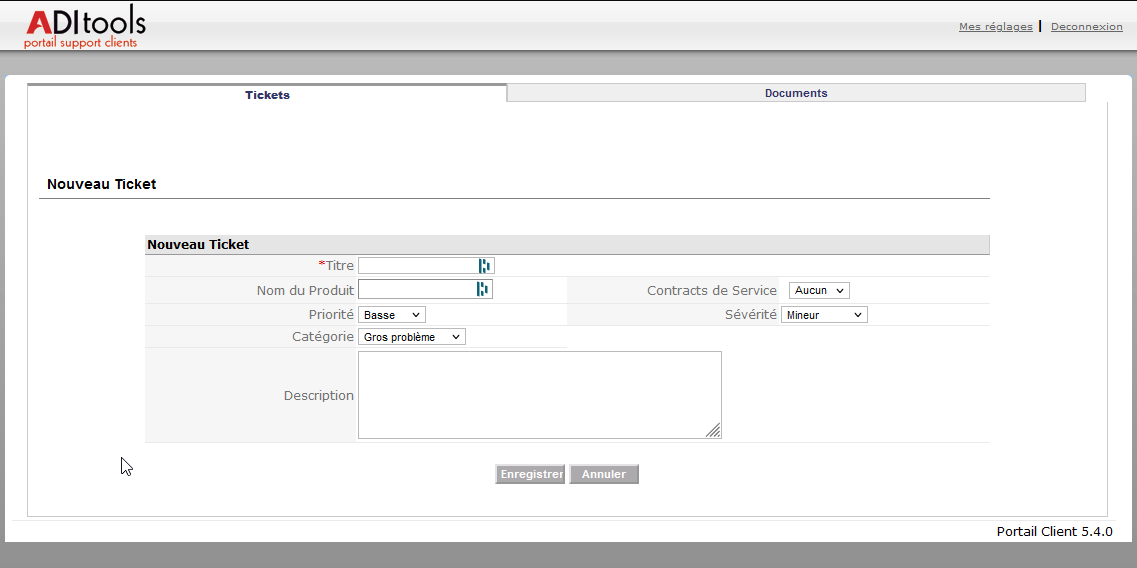
\includegraphics[width=6.3in,height=3.14722in]{image2.png}

% On peut constater que l'interface est plutôt minimaliste et
% vieillissante. Il manque certaines fonctions qui seront abordées plus
% bas.

% \textbf{Nouveau logiciel souhaité}

% Nous souhaitons migrer vers un nouveau logiciel de ticketing qui puisse
% intégrer les fonctionnalités ci-dessous~:

% Création d'incidents

% \begin{quote}
% La gestion des incidents permet de suivre et de résoudre les incidents
% signalés par les utilisateurs.
% \end{quote}

% Création de demandes de changement

% \begin{quote}
% Gestion des changements permet de planifier, suivre et gérer les
% modifications demandées par les utilisateurs.

% Exemple~: modification de ports sur le firewall, augmenter une boite aux
% lettres, etc.
% \end{quote}

% Création de tickets automatiquement

% \begin{quote}
% Cette fonctionnalité permet de planifier des interventions récurrentes
% sans les oublier. Exemple~: test de restauration
% \end{quote}

% Gestion des ressources

% \begin{quote}
% Pouvoir lié du matériel ou logiciel a un client et faire un suivi des
% modifications sur ce cette ressource.

% Exemple~: avoir le suivi des modifications comme celui qui est présent
% sur la page client du wiki.

% Intégrer du matériel lié à un fournisseur et gérer sa garantie. Exemple
% NAS ANANDA.

% Gérer les renouvellements~: des certificats

% Gérer les renouvellements~: des noms de domaines
% \end{quote}

% Inventaires

% \begin{quote}
% Lister l'ensemble des machines (connecteur OCS)
% \end{quote}

% Tableaux de bord et rapports

% Avoirs des stats et indicateurs sur ce qui nous prend le plus de temps
% dans le support.

% Ergonomique

% \begin{quote}
% Il faut que le logiciel soit intuitif et ergonomique. Que l'utilisateur
% ne soit pas rebuté par la complexité d'ouverture d'un ticket.
% \end{quote}

% Ouverture de ticket via email

% Fermeture de ticket automatique après un délai de non-réponse

% Personnalisation graphique

% \begin{quote}
% Nous souhaitons que l'application puisse se personnaliser aux couleurs
% de la société et d'y insérer le logo.
% \end{quote}

% Récupération des données ticketing vtiger

% \begin{quote}
% Seulement si cette récupération est facile. Ne pas perdre du temps sur
% cette récupération.
% \end{quote}

% Fonctions annexes

% Gestion des baies racks du datacenter

    
    % Pós Textuais
    % \nocite{*}
    % \include{pos-textuais/referencias}

\end{document}
